\chapter{Experiments and Results}
\label{chap:ExperimentsAndResults}

TODO: quick chapter overview

\begin{code}
$ python3 main.py unet train --val_pages 123 ...
\end{code}


\section{Architecture}
\label{sec:Architecture}


\section{Datasets}
\label{sec:Datasets}


\section{Semi-supervised Improvements}
\label{sec:SemisupervisedImprovements}

The main hypothesis this work is attempting to validate is that adding unlabelled data to the training process helps. We primarily want to improve model accuracy, but as we will see, this is not what the experiments suggest. They do, however, show improvements in other areas, such as training stability and reduced overfitting (section \ref{sec:UtilizingCvcMuscima}).

In the first experiment, we test how various labeled to unlabeled data ratios affect the training process. The experiment uses the MUSCIMA++ dataset [CITE]:

\begin{itemize}
    \item 10 pages act as the labeled set.
    \item 0, 5, 10 and 50 pages act as the unlabeled set.
    \item 10 pages act as the validation set.
    \item All of these pages come from the writer-independent train set of MUSCIMA++ and are chosen in a writer-independent manner (all three splits contain pages by different writers).
\end{itemize}

The learned task is notehead segmentation (both full and empty noteheads). Noteheads are an ideal symbol for this kind of measurement. Firstly, they are very abundant. Each page of the dataset contains many instances of them and they are evenly scattered over the whole page. If we were to instead detect more rare symbols (such as clefs or rests), it could skew the results, making it difficult to separate the effects we want to measure. Handwritten noteheads are also very diverse in style, making them more interesting to learn (compared to, say, stafflines).

All model hyperparameters are set to sensible deafults. The derivation of these values is desribed later in section \ref{sec:UnderstandingHyperparameters}. The proposed dataset is rather small and so the training is very noisy (figure \ref{fig:ExplorationNoteheadsNoDropout}). To stabilize the trainig we set the dropout parameter to 50\% [CITE DROPOUT].

\begin{figure}[ht]
    \centering
    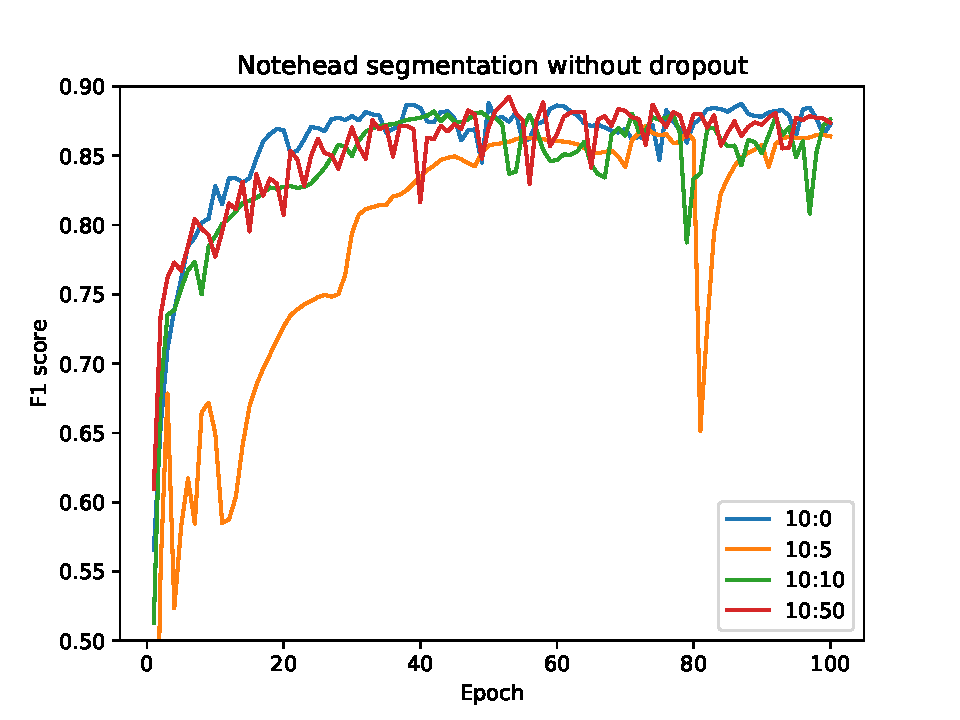
\includegraphics[width=140mm]{../../figures/01-exploration-noteheads/noteheads.pdf}
    \caption{Training on a small dataset without dropout is noisy, see the orange line at the beginning and the green line at the end.}
    \label{fig:ExplorationNoteheadsNoDropout}
\end{figure}

We expect that as we add more and more unlabeled data, the F1 score should reach higher and higher. Or at least not get worse. This is not what we see in the chart \ref{fig:ExplorationNoteheads}. The fully supervised model outperforms all the others by a clear margin.

Focusing only at the semi-supervised models, it seems that adding more unsupervised data maybe helps here, although the three lines end up on top of each other at the epoch 200. A better idea is to look at the table \ref{tab:ExplorationNoteheads}. TODO: popiš že tabulka obsahuje testovací f1 skóre a že je to přes několik běhů a výsledek je? (snad bude vzestupný trend a když ne, tak komentuj, že je to totálně random)

The reason for the drop in performance is actually caused by the fact, that the supervised model has to only learn one task -- segmentation. Whereas the semi-supervised one has to also learn the unsupervised reconstruction task. This claim is explored in the next section and is supported by the fact that the performance drop disappears when we increase model capacity.

\begin{figure}[p]
    \centering
    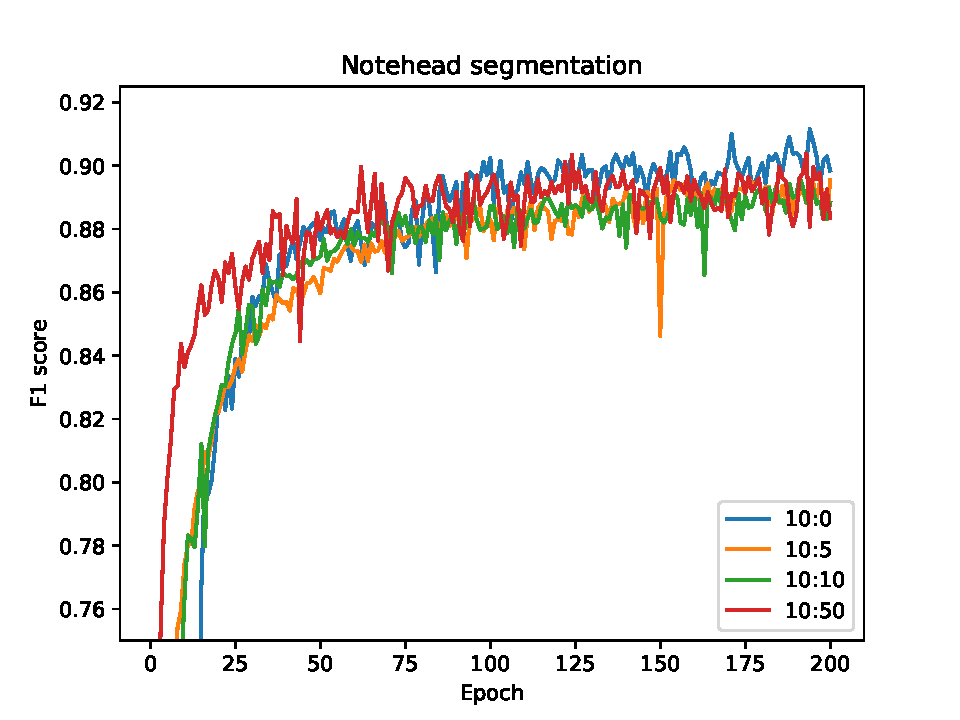
\includegraphics[width=140mm]{../../figures/01-exploration-noteheads/noteheads-dropout.pdf}
    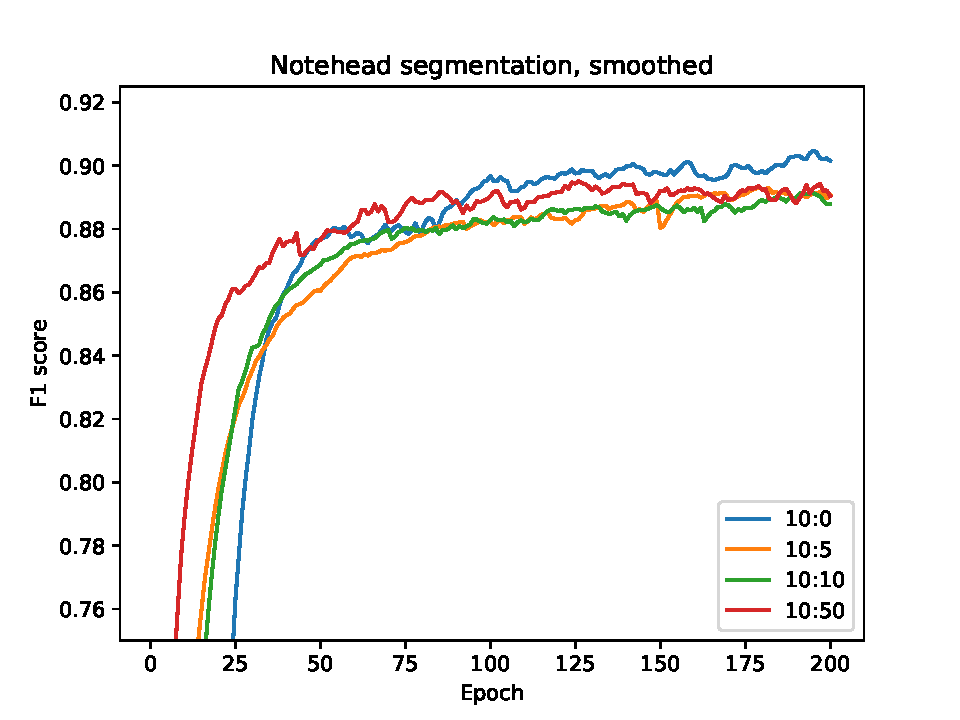
\includegraphics[width=140mm]{../../figures/01-exploration-noteheads/noteheads-dropout-smooth.pdf}
    \caption{Lorem ipsum dolor.}
    \label{fig:ExplorationNoteheads}
\end{figure}

\begin{table}[b!]
    \centering
    \begin{tabular}{l@{\hspace{1.5cm}}D{.}{,}{3.2}D{.}{,}{1.2}D{.}{,}{2.3}}
        \toprule
        & \mc{} & \mc{\textbf{Směrod.}} & \mc{} \\
        \pulrad{\textbf{Efekt}} & \mc{\pulrad{\textbf{Odhad}}} & \mc{\textbf{chyba}$^a$} &
        \mc{\pulrad{\textbf{P-hodnota}}} \\
        \midrule
        Abs. člen     & -10.01 & 1.01 & \mc{---} \\
        Pohlaví (muž) & 9.89   & 5.98 & 0.098 \\
        Výška (cm)    & 0.78   & 0.12 & <0.001 \\
        \bottomrule
    \end{tabular}
    \caption{Lorem ipsum dolor.}
    \label{tab:ExplorationNoteheads}
\end{table}

TODO: show visualization images / qualitative comparison between runs?


\section{Utilizing CVC-MUSCIMA}
\label{sec:UtilizingCvcMuscima}





TODO: maybe an experiment? Small model (2ft) on small dataset (few pages) - unsueprvised data helps stabilize training instead of dropout. (file diplomka-inner-features.odt)

\section{Understanding Hyperparameters}
\label{sec:UnderstandingHyperparameters}


\subsection{Batch Size}

\subsection{Dropout}

\subsection{Skip Connections}

\subsection{Unsupervised Loss Weight}

\subsection{Activation Function}
